\begin{BlueBox}
    \vskip-1cm
    \begin{block}{\BHead{Background}}
        \begin{itemize}
            \item Temperature main meteorological driver of surface ozone in many areas. \vspace{12mm}
            \item Temperature \vspace{6mm}
                \begin{itemize}
                    \item increases isoprene emissions from vegetation, \vspace{4mm}
                    \item increases reaction rates of chemical processes.  \vspace{12mm}
                \end{itemize}
            \item VOC the ``fuel'' and \ce{NO_x} the ``catalyst'' of ozone production. \vspace{12mm}
        \end{itemize}
        \vspace{5mm}
        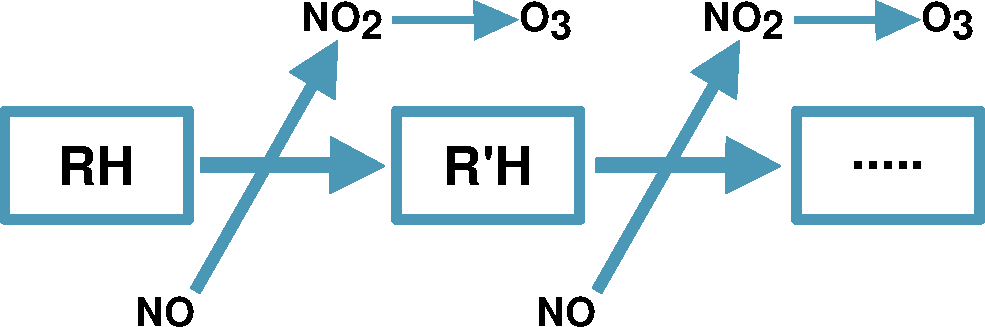
\includegraphics[width=\textwidth]{VOC_Oxidation} \vspace{5mm}
        \begin{itemize}
            \item What drives the ozone--temperature relationship? Increased isoprene emissions or chemistry? \vspace{12mm}
            \item Can chemical mechanisms simulate the ozone--temperature relationship across \ce{NO_x} gradients? \vspace{12mm}
        \end{itemize}
    \end{block}
\end{BlueBox}
